% !TEX encoding = UTF-8 Unicode
\graphicspath{{figuras/}}
\chapter{Critérios de avaliação} \label{cap5}
Trabalhos orientados como o desenvolvimento de estágios técnicos supervisionados, projetos de graduação de conclusão de curso  ou   iniciação científica e tecnológica  são avaliados por meio da documentação técnica produzida na forma de relatório ou artigo (\cite{Markel1994}).  Além disso, no caso de projeto final de curso, normalmente há uma avaliação oral, realizada por uma banca examinadora durante sessão pública. Os critérios de avaliação são variados e muitas vezes modulados por aspectos subjetivos dos avaliadores. A seguir são apresentadas duas tabelas que relacionam critérios com ponderações típicas, uma para avaliação de um texto técnico e outra para uma sessão de apresentação oral cujo objetivo é minimizar discrepâncias de avaliação e prover critérios objetivos que ao serem antecipados permitem otimizar a pontuação da atividade. Dicas para preparar slides são fornecidas no final.
\section{Tabela de avaliação do relatório técnico}
% --- Figura simples TikZ
\keyfigbox[W]{wlw=0.35,c={Janela de Johari.},l=fig:JohariWindow, t={É uma técnica que ajuda as pessoas a compreenderem seu relacionamento com elas mesmas e com os outros. Quando somos avaliados muitas vezes descobrimos coisas que normalmente não enxergamos em nós mesmos e no nosso trabalho. }}{%--- Inicio
	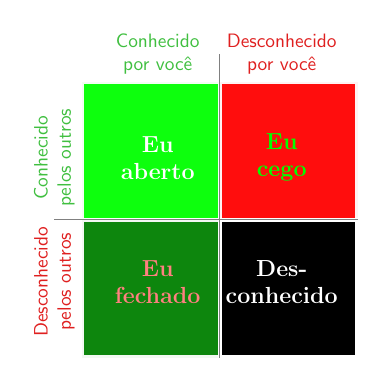
\begin{tikzpicture}[scale=0.7, transform shape]
		\filldraw[ultra thick,white,fill=green, opacity=0.95]rectangle ++(-2.5,2.5);
		\node at (-1.125,1.125) [align=center, text width=2.5cm, font=\large]{\color{white}\textbf{Eu\\ aberto}}; 
		
		\filldraw[ultra thick,white,fill=green!50!black, opacity=0.95] (0,0) rectangle ++(-2.5,-2.5);
		\node at (-1.125,-1.125) [align=center, text width=2.5cm, font=\large]{\color{red!50}\textbf{Eu\\ fechado}}; 
		
		\filldraw[ultra thick,white,fill=red, opacity=0.95] (0,0) rectangle ++(2.5,2.5);
		\node at (1.125,1.125) [align=center, text width=2.5cm, font=\large]{\color{green}\textbf{Eu\\ cego}}; 
		
		\filldraw[ultra thick,white,fill=black, opacity=1] (0,0) rectangle ++(2.5,-2.5);
		\node at (1.125,-1.125) [align=center, text width=2.5cm, font=\large]{\color{white}\textbf{Des-conhecido}}; 
		
		\draw[thin,gray] (0,-2.5) --++(0,5.5);
		\draw[thin,gray] (-3,0) --++(5.5,0);
		%--- você mesmo
		\node[align=center, text width=2.5cm] at (-1.125,3) {\color{green!50!gray}\textsf{Conhecido por você} };
		\node[align=center, text width=2.5cm] at (1.125,3) {\color{red!75!gray}\textsf{Desconhecido por você} };
		
		%--- os outros
		\node[align=center, text width=2.5cm,rotate=90] at (-3,1.125) {\color{green!50!gray}\textsf{Conhecido pelos outros} };
		\node[align=center, text width=2.5cm, rotate=90] at (-3,-1.125) {\color{red!75!gray}\textsf{Desconhecido pelos outros} };
	\end{tikzpicture}
}
Somos avaliados, geralmente, para recebermos uma nota pelo trabalho realizado e para classificar uma atividade em determinado contexto. O mais importante é saber que avalia-se alguém para  \emph{conhecer}, \emph{valorizar} e \emph{responsabilizar}. Como ilustrado na Figura~\ref{fig:JohariWindow}, ao sermos avaliados temos a oportunidade de descobrirmos coisas desconhecidas em nós mesmos e no nosso trabalho. Para tanto, é muito  importante que saibamos a priori, como seremos avaliados e quais são os critérios objetivos.  Desta forma podemos evitar aborrecimentos e otimizar nossos esforços para obter uma boa avaliação.  Neste sentido,  é essencial conhecer e refletir sobre os tópicos normalmente avaliados por uma banca examinadora ao se iniciar um projeto para que, desde o início, sejam considerados todos os aspectos pertinentes que porventura venham a ser avaliados apenas ao término do trabalho ou projeto. 
A seguir apresentam-se as  tabelas \ref{tab:CriteriosAvalMonog} e  \ref{tab:CriteriosAvalSeminario} com sugestões ponderadas de critérios usados numa avaliação de projetos acadêmicos. As ponderações e os respectivos critérios servem para guiar e elucidar variados aspectos essenciais desde a fase de elaboração de uma proposta, até a documentação do desenvolvimento das atividades e  a produção de um texto técnico.
\clearpage
%%%%%%%%%%%%%%%%%%%%%%%%%%%%%%%%%%%%%%%%%%
 \DefTblrTemplate{contfoot-text}{default}{Continua na página seguinte$\ldots$}
\DefTblrTemplate{conthead-text}{default}{(continuação)}
\begin{longtblr}[
	%	theme = fancy,
	caption = {Critérios de avaliação de monografias.},
	label = {tab:CriteriosAvalMonog},
	note{$\dag$} = {Os valores percentuais de peso indicados em cada questão representam o valor máximo da questão. A coluna Máx. contém a nota máxima recomendada para cada item de uma questão.},
	]{%
		width=1.1\linewidth,
		hlines={black},
		vlines={gray!50},
		rowhead=1,
		row{1}=  {bg=azure3,  fg=white,  font=\sffamily},
		colspec={Q[c,h,-1]  Q[l,h,5]  Q[l,h,7]  Q[c,m,-1]  Q[c,m,-1]},
		cell{1}{1} = {r=1,c=2}{c,m},
		cell{1}{3} = {r=1,c=1}{c,m},
		cell{3}{1} = {r=2,c=1}{l,h},		cell{3}{2} = {r=2,c=1}{l,h}, 
		cell{5}{1} = {r=8,c=1}{l,h},		cell{5}{2} = {r=8,c=1}{l,h}, 
		cell{13}{1} = {r=3,c=1}{l,h},		cell{13}{2} = {r=3,c=1}{l,h}, 
		cell{16}{1} = {r=6,c=1}{l,h},		cell{16}{2} = {r=6,c=1}{l,h}, 
		cell{22}{1} = {r=7,c=1}{l,h},		cell{22}{2} = {r=7,c=1}{l,h}, 
		cell{29}{1} = {r=7,c=1}{l,h},		cell{29}{2} = {r=7,c=1}{l,h}, 
		cell{36}{1} = {r=2,c=1}{l,h},		cell{36}{2} = {r=2,c=1}{l,h}, 
	}
	Questão  &    &  Critérios  de  avaliação  & {\rotatebox[origin=c]{90}{Máx.${}^{\dag}$} } &  {\rotatebox[origin=c]{90}{Nota}}  \\  
	
	1  &{\fbox{Peso = 2\%} \\ O  título  da  monografia  descreve  apropriadamente  o  \emph{assunto}  e  a  \emph{proposta}?} &  {Avaliar considerando  a  pertinência da abordagem  e  dos  tópicos  apresentados. \\ Avaliar  se  o  título  é: \\ $\bullet$ Suficientemente  preciso,\\ $\bullet$ Fácil  para  ler  e  entender,  e \\ $\bullet$ Estruturado  para  o  tema  e  a  audiência.} & 3   &   \\  
	2  & {\fbox{Peso = 6\%} \\ O  Abstract  apresenta  um  resumo  sucinto  do  trabalho  contendo  o  assunto,  a  proposta  e  o  escopo,  servindo  como  um  guia  para  a  leitura  da  monografia?}  &  {O  resumo  da  monografia  deve  responder  adequadamente  às  seguintes  questões: \\ 2.1     Qual  é  o  assunto,  a  proposta  e  o  escopo  do  trabalho? } &  3  &    \\  
	&    &  2.2     Quais  são  os  pontos  mais  importantes  apresentados  no  texto?  &   3 &       \\  
	3  &{\fbox{Peso = 15\%} \\ As  características  essenciais  de  um  texto  técnico  profissional (\cite{Markel1994}) foram  adequadamente  respeitadas? }
	&  3.1   Clareza:  o  texto  deve  proporcionar  condições  de  entendimento  ao  leitor.  Avaliar  citação  e  comentários  no  texto  para  figuras,  equações  e  referências  bibliográficas.  Todos  estes  itens  devem  ser  devidamente  comentados  no  texto  principal.  &  4  &   \\  
	&   & 3.2  {Honestidade:  Informar corretamente a  origem,  desenvolvimento  e  autoria  das  ideias.  Avaliar  o  excesso  ou  omissão  de  referências  bibliográficas  com  a  presença  ou  uso  de  citações  inadequadas. } & 3   &     \\  
	&    &  3.3     Correção:  o  autor  deve  respeitar  as  regras  de  escrita  culta,  referentes  à  gramática,  ortografia,  acentuação,  estilo,  etc.  Avaliar  a  existência  de  erros  grosseiros  e  repetitivos  de  acentuação  e  ortografia.  Uso  exagerado  e  desnecessário  de  estrangeirismos.  &  3 &    \\  
	&    &  3.4    Exatidão:  apresentar  os  fatos  e  os  dados  como  eles  são,  corretamente.  Inexatidões  são,  no  mínimo,  confusas  e  aborrecidas,  podendo  ser,  também,  perigosas  (pode  gerar  suspeita  de  manipulação  intencional  dos  dados).  &  1  &    \\  
	&    &  3.5    Acessibilidade:  o  texto  deve  ser  estruturado  para  facilitar  ao  leitor  a  localização  da  informação  que  ele  precisa.  &  1  &  \\  
	&    &  3.6     Compreensividade:  o  texto  deve  conter  todas  as  informações  de  que  o  leitor  precisa  ou,  pelo  menos,  referências  cruzadas  de  outros  documentos  pertinentes.  &  1  &    \\  
	&    &  3.7      Concisão:  o  texto  deve  ser  tão  conciso  quanto  possível,  respeitando-se  os  demais  critérios  sem  sacrificá-los.  Textos  prolixos  demais  são  cansativos  e  desmotivadores  para  o  leitor.  &  1  &    \\  
	&    &  3.8       Diplomacia:  o  autor  deve  ser  educado  e  delicado  ao  escrever  para  evitar  conflitos  e  resultados  desnecessários  e  indesejáveis.  &  1  &    \\  
	4  &  {\fbox{Peso = 7\%} \\  O  capítulo  de  introdução  contextualiza  o  tema,  justifica  a  relevância  e  apresenta  objetivos  específicos  para  a  monografia?}  &  4.1     Contextualização  do  tema  &  2  &    \\  
	&    &  4.2       Justificativa  técnica  do  tema  &  3  &   \\  
	&    &  4.3       Descrição  dos  objetivos  específicos  e  gerais  da  monografia  &  2  &     \\  
	5  &  { \fbox{Peso = 8\%} \\ A  monografia  contempla  uma  revisão  bibliográfica  pertinente  ao  tema,  atualizada  e  orientada  cientificamente  com  contextualização  crítica  (não  apenas  resumo)  do  autor  da  monografia? \\
		Considerar  para  cada  índice: Muito  Pobre  ou  Inaceitável  0\% ; Insuficiente  5\% ; Suficiente  10\% ; Adequado  15\%; Avançado 20\%}   &  {As  Referências  Bibliográficas  contemplam:\\ 
		5.1    Fontes  que  abordam  os  princípios  e  fundamentos  teóricos  e  tecnológicos  envolvidos  no  tema,  bem  como  trabalhos  correlatos  já  desenvolvidos  ou  em  desenvolvimento.}  &  3  &     \\  
	&    &  5.2     Uma  única  ou  poucas  fontes  ($<3$  é  inaceitável)  & 1  &   \\  
	&    &  5.3     Predominância  de  livros  textos  didáticos  ($>60\%$ é  inaceitável);  & 1   &    \\  
	&    &  5.4     Referências  a  um  único  grupo  de  pesquisa  ou  empresa  ($<3$  é  insuficiente);  &  1  &    \\  
	&    &  5.5    Referências  com  predominância  de  sítios  da  internet  e  sem  rastreamento  assegurado  ($>50\%$  é  muito  pobre e inaceitável);  &  1 &  \\  
	&    &  5.6    Documentos  de  acesso  restrito  e  sem  revisão  técnica  de  corpo  editorial  (revistas)  ou  técnico-profissional  (normas  técnicas  de  órgãos  oficiais)  ($>50\%$  é  inadequado)  & 1   &    \\  
	6  &  {\fbox{Peso = 7\%} \\  
		Os  capítulos  apresentam  um  desenvolvimento  de  tópicos  pertinentes  ao  tema  e  encadeados  logicamente? \\
		A  monografia  apresenta um  texto  coeso  (harmônico,  associado,  lógico,  coerente)  ao invés de uma  coletânea  de  textos  e  informações  “soltas”?\\ \vspace{0.5cm}
		\emph{Avaliar considerando  um  público  alvo  para  a  monografia  com  embasamento  teórico  técnico ou de engenharia.}}&  {
		6.1   Encadeamento  lógico:  Introdução,  Detalhamento,  Análise  de  Resultados,  Comentários  finais  e  Sugestões  de  trabalhos  futuros. } & 3   &     \\  
	&    & { 6.2  Delineamento  (assunto,  proposta,  escopo)  do  tópico  abordado  em  cada  capítulo.}  &  1  &   \\  
	&    &  {6.3  Dissertação  com  a  pessoa  da  narrativa  mantida  em  todo  texto  (impessoal  é  desejável  e  usual). } &  1  &     \\  
	&    & { 6.4     Itemização  com  paralelismo  de  linguagem  (itens  no  mesmo  estilo)  mantido. }&  0.5  &   \\  
	&    &  6.5    \ Uso  exagerado  de  jargões,  siglas  sem  descrição  implicando  em  dificuldade  de  compreensão  do  tema  abordado  e  omissão  de  lista  de  nomenclatura.  & 0.5   &   \\  
	&    &  6.6   { Apresentação  de  dados  em  gráficos  com  eixos  e  títulos  devidamente  identificados  com  variáveis  e  parâmetros  objetivos  adequados  para  análise? \\ (\emph{Dados  +  Interpretação  =  Inteligível}) } &  0.5  &   \\  
	&    &  {6.7    Uso  adequado  de  tempos  verbais,  prevalecendo  o  tempo  presente  para  as  características  com  sentido  de  atemporalidade,  e.g.  “...será  apresentado  no  capítulo  X”  ao  invés  do  recomendado  “...é  apresentado  no  capítulo  X”.} & 0.5   &    \\  
	7  &  {\fbox{Peso = 40\%}\\ As características  do  trabalho  são compatíveis  com   as  etapas  do  desenvolvimento,  resultados  obtidos  e  analisados?  Avaliar  4  itens  ou  a  média  ponderada  de  mais  itens  se  for  o  caso,  dentre  os  apresentados  de  acordo  com  o  enfoque  do  trabalho até o limite de $20\%$.}  &  7.1     Detalhamento  ou  memorial  descritivo  de  projeto  de  engenharia  utilizado  como  objeto  no  trabalho  apresentado  na  monografia;  &  10  &   \\  
	&    &  7.2   Estudo  de  caso(s)  específico(s)  com  levantamento  de  dados  de  campo;  &  10 &    \\  
	&    &  7.3   Obtenção  e  análise  de  dados  experimentais  (monitoramento,  ensaios,  etc.).  Foi  detalhada  a  obtenção  dos  dados  (de  terceiros,  próprios,  públicos,  restritos,  etc.)?  &  10  &    \\  
	&    &  7.4   Obtenção  e  análise  de  dados  de  simulação,  estudo  de  casos  com  respectivas  hipóteses,  restrições,  simplificações  e  aproximações  específicos  para  o  tema  da  monografia;  &  10  &     \\  
	&    &  7.5    Avaliação  de  desempenho  ou  resultados  de  programas  desenvolvidos  especificamente  no  trabalho  de  graduação;  &  10  &   \\  
	&    &  7.6   Detalhamento  de  diagramas  esquemáticos  de  circuitos  (eletro-eletrônico,  pneumático,  hidráulico,  mecânico,  térmico,  de  instrumentação,  lógico,  fluxogramas,  etc.),  montagens,  arranjos  experimentais  e  ensaios  de  protótipos?  &  10 &    \\  
	&    & { 7.7    Outros.  Favor  especificar\\  \vspace{1cm}  }&  10 &   \\  
	8  &  {\fbox{Peso = 8\%}\\  Os  Comentários  Finais ou  Conclusões  e  as  Sugestões  de  Trabalhos  Futuros  têm  correlação  com  o  trabalho  descrito  no  corpo  da  monografia? \\ \emph{No capítulo das  conclusões    alinhavam-se os resultados já descritos anteriormente, sendo não recomendado fornecer informações  novas  não  comentadas  ou  não examinadas previamente.}}  & 
	{8.1  As  conclusões   versam  sobre:\\
		$\bullet$  O  que  foi  feito  e  descrito  na  monografia.\\
		$\bullet$  Os  pontos  fortes  do  trabalho.\\ 
		$\bullet$  Todos  os  objetivos  propostos  e  como  foram  alcançados}  &  5  &    \\  
	&    &  
	{8.2    As  sugestões  de  trabalhos  futuros\\
		$\bullet$  Demonstram  visão  do  que  foi  feito  e  o  que  ainda  pode  ou  precisa  ser  feito?\\
		$\bullet$  Exageram  deixando  a  impressão  de  que  o  trabalho  principal  ainda  precisa  ser  feito? } & 3   &   \\  
	9  &  {\fbox{Peso = 2\%}\\ Os  Agradecimentos foram  feitos  com  pertinência  e  honestidade?  }&  {Verificar  se  o  trabalho  utilizou  recursos  e  informações  de: \\
		$\bullet$Agências  de  fomento,\\
		$\bullet$ Orientadores/Departamento,\\
		$\bullet$ Supervisores/Empresa, \\
		$\bullet$ Laboratórios/grupos  de  pesquisa}  &  2 &   \\  
	10  &  {\fbox{Peso = 5\%}\\ Avaliação  global  do  trabalho  apresentado  na  monografia.\\ 
		$\bullet$ Inaceitável  0\%;  \\ 
		$\bullet$ Insuficiente  $<40\%$; \\ 
		$\bullet$ Suficiente  $60\%$  a  $75\%$;\\ 
		$\bullet$ Adequado  $75\%$  a  $90\%$; \\ 
		$\bullet$ Avançado  $90\%$  a  $100\%$.}&  O  estudante  demonstrou,  desenvolveu  ou  aprimorou  com  o  trabalho  de  graduação  características  essenciais  de  um  profissional  tais  como  objetividade,  iniciativa,  persistência,  determinação,  dedicação,  capacidade  de  síntese  e  comunicação  técnica  adequada?  &  5  &     \\ 
	&  Avaliação  da Monografia & Nota $M$   & {\color{gray}100}  &  \\  
\end{longtblr}



\section{Tabela de avaliação do seminário de defesa}
\begin{longtblr}[
	%	theme = fancy,
	caption = {Critérios de avaliação do seminário de defesa.},
	label = {tab:CriteriosAvalSeminario},
	note{$\dag$} = {Os valores percentuais de peso indicados em cada questão representam o valor máximo da questão. A coluna Máx. contém a nota máxima recomendada para cada item de uma questão.},
	]{%
		width=1.1\linewidth,
		hlines={black},
		vlines={gray!50},
		rowhead=1,
		row{1}=  {bg=azure3,  fg=white,  font=\sffamily},
		colspec={Q[c,h,-1]  Q[l,h,5]  Q[l,h,7]  Q[c,m,-1]  Q[c,m,-1]},
		cell{1}{1} = {r=1,c=2}{c,m},
		cell{1}{3} = {r=1,c=1}{c,m},
		cell{2}{1} = {r=7,c=1}{l,h},		cell{2}{2} = {r=7,c=1}{l,h}, 
		cell{9}{1} = {r=6,c=1}{l,h},		cell{9}{2} = {r=6,c=1}{l,h}, 
	}
	Questão  &    &  Critérios  de  avaliação  & {\rotatebox[origin=c]{90}{Máx.${}^{\dag}$} } &  {\rotatebox[origin=c]{90}{Nota}}  \\  
	1 &  {\fbox{Peso = 35\%}\\  O  seminário  ministrado  contemplou  os  elementos  básicos  de  uma  apresentação  técnica? \\\vspace{1cm}  \emph{Recomenda-se   apresentar  a  solução  ou  resultados  finais  obtidos no início. para despertar a curiosidade da audiência e evitar de estourar o tempo sem apresentar o melhor resultado!} } &  1.1  {Introdução com contextualização  do  assunto  e  da  proposta.}  &   5 &     \\  
	&    &  1.2   Revisão  da  literatura  e  fundamentos  teóricos  &  5  &     \\  
	&    &  1.3   {Descrição  do  trabalho \\
		$\bullet$  Diagramas,  esquemas,  circuitos,  fluxogramas,  formulações  matemáticas,  etc.  }&  5  &  \\  
	&    &  1.4  Estudo  de  caso:  Simulação,  descrição  de  operação  de  sistemas,  descrição  de  modos  de  operação,  aplicações  e  usos.  &  5&    \\  
	&    &  {1.5 Empacotamento  da  solução\\
		$\bullet$  Algoritmos  ou  rotinas  de  computador\\
		$\bullet$  Projeto  conceitual  ou  memorial  descritivo\\
		$\bullet$  Plano  de  obras  e  implantação,  etc. } &  5  &    \\  
	&    &  {1.6  Resultados\\
		$\bullet$  Análise  e  comentários  sobre  dados  experimentais,  de  simulação  ou  levantamento  de  campo  como  construído  (as  built),  etc.  }&  5  &    \\  
	&    &  {1.7  Epílogo: \\
		$\bullet$ Comentários  finais  e  sugestões  para  trabalhos  futuroso \\
		$\bullet$ Perguntas  e  respostas\\
		$\bullet$ Outros  (agradecimentos; referências  bibliográficas  destacadas. } &  5 &     \\  
	2  &  {\fbox{Peso = 65\%}\\ 
		O  seminário foi apresentado olhando  para os ouvintes,  com  clareza  na  explanação  das  ideias,  domínio  do  conteúdo  e  respostas  adequadas  às  indagações  da  banca? } &  
	2.1  {A  apresentação  foi  bem  dimensionada  e  administrada  para  o  tempo  previsto ($\approx 30min$)? \\ 
		O  aluno  demonstrou  ter  se  preparado  adequadamente,  ensaiado  e  cronometrado  o  tempo  da  apresentação?\\ } &  10  &   \\  	&    &  
	2.2  {Os  slides  foram  preparados  adequadamente  para  serem  apreciados  em  bom  tempo  (2min/slide)  pela  audiência? \\
		Para  balizar  a  avaliação  considere  uma  apresentação  objetiva  e  legível  como  sendo  composta  de  \emph{slides}  com:  (i) seis  palavras  por  linha; (ii)  seis  linhas  por  slide.  Um  \emph{slide}  bem  escrito  usa  o  paralelismo  de  linguagem,  por  exemplo:\\
		$\bullet$  Escrever  corretamente\\
		$\bullet$  Revisar  periodicamente\\
		$\bullet$  \xout{Opção de contingência}. \\
		$\bullet$   Preparar opção de contingência.}  &  5  &   \\  
	&    &  {2.3  Dados  foram  apresentados  em  gráficos  com  eixos  e  títulos  devidamente  identificados  com  variáveis  e  parâmetros  objetivos  adequados  para  análise?\\
		As  figuras  foram  devidamente  identificadas  e  ilustraram  aspectos  pertinentes? } &  10  &    \\  
	&    &  {2.4   O  apresentador  demonstrou  uma  postura  adequada,  direcionando  a  fala  para  os  presentes  ao  invés  da  tela,  paredes,  janelas,  etc.?\\
		Observar  que  limitações  de  fala  ou  visão  não  devem  ser  avaliadas,  mas  sim  a  postura  e  a  determinação  em  se  fazer  entender.}  & 5   &    \\  
	&    &  {2.5   As  falas  foram  decoradas  ou  meramente  lidas  ou  foram  interpretadas  demonstrando  domínio  de  conteúdo?}  &  5 &   \\  
	&    &  {2.6    As  questões  da  banca  referentes  ao  tema  do  trabalho  foram  respondidas  satisfatoriamente?Favor  comentar}  &  30  &  \\  
	3  &  Avaliação  do Seminário & Nota $S$   & {\color{gray}100}  &  \\  
\end{longtblr}
\section{Avaliação Final}
	Avaliar é uma etapa de correção de abordagens, uniformização de estilos, completando a necessária adequação formal típica para uma publicação técnica. A avaliação final é a soma algébrica das notas em cada questão avaliada, desde que sejam respeitados os limites máximos para cada item pontuado. Se o trabalho é avaliado em duas etapas, i.e. relatório técnico ou monografia (nota $M$) e avaliação do seminário (nota $S$), a nota final, $N_F$, deve ser uma média ponderada dessas avaliações:
	\begin{equation}
		N_F =\alpha \, M + (1-\alpha)\, S,
	\end{equation}
	em que $\alpha$ pondera o texto técnico complementarmente ao seminário. O valor usual sugerido para $\alpha =0.6$ pondera com 60\% o texto técnico e a apresentação do seminário com 40\%. Dessa forma, a parte mais trabalhosa de redação técnica é  valorizada 50\% a mais que a avaliação do seminário. Todavia, como a apresentação é um sumário do trabalho realizado,  é comum durante a sessão de avaliação oral serem fornecidas visões e interpretações integradas dos resultados produzidos que esclarecem pontos obscuros ou  pouco claros no relato técnico. Assim, as ponderações de 60\% e 40\% são uma sugestão,  que devem ser ajustadas para cada contexto. O importante é que ao registrar notas para diferentes aspectos do trabalho, são fornecidos realimentações para as usuais correções subsequentes do trabalho, antes de ser publicado e arquivado. As sugestões de avaliação são apenas um guia para focar  os diferentes aspectos de uma redação técnica, permitindo uma avaliação justa (igual para todos) e objetiva, que contribui para o aprimoramento do documento a ser publicado. 
	
\section{Sugestões para composição de uma apresentação com slides}

A apresentação do seminário é usualmente amparada por slides. Preparar slides profissionalmente requer tempo e organização. Antes de apresentar recomendações é  importante ressaltar que, infelizmente,  notas de aula de professores não são, em geral,  uma  referência adequada para extrair ideias de como estruturar slides. Professores tendem a usar slides como resumo de notas de aula e isso resulta em slides sobrecarregados e com excesso de informação. Tudo que deve ser evitado ao máximo ao preparar uma apresentação clara, e inteligível. Para piorar, é bom saber que  slides que são preparados para atender  a dois propósitos (apresentação e resumo de conteúdo como notas de aula) não atendem nem um nem outro. Então, embora os avaliadores sejam geralmente professores, os slides não devem seguir o padrão usual  destes! 

A primeira coisa a saber é que seres humanos normalmente organizam e interpretam ou contabilizam com facilidade até seis itens de uma vez. Pouquíssimas pessoas conseguem reconhecer, agrupar e acompanhar mais que seis itens no espaço de um slide, portanto, a \emph{métrica alvo de ouro}  é \textbf{escrever slides com 6 linhas e 6 palavras por linha}. A Figura~\ref{fig:slidesLeves6x6} ilustra um slide que extrapola ligeiramente esta métrica de ouro, mas que ainda assim é legível. 

\keyfigbox[H]{f,lw=1, c={Dicas para elaborar slides $6 \times 6$ inteligíveis.}, l=fig:slidesLeves6x6}{% --- inicio
	\textbf{Dicas}
	\begin{itemize}[noitemsep]
		\item Uma apresentação objetiva e legível tem 
		\subitem $\bullet$ Seis palavras por linha
		\subitem $\bullet$ Seis linhas por slide.
		\item Um slide bem escrito usa o paralelismo de linguagem:
		\subitem $\bullet$  Escrever  corretamente
		\subitem $\bullet$  Revisar  periodicamente
		\subitem $\bullet$  \xout{Opção de contingência}. 
		\subitem $\bullet$   Preparar opção de contingência.
		\item Uma análise de Impacto x Custo ajuda o leitor a entender as prioridades.
		\item Uma opção de contingência preparada a priori
evita supresas desagradáveis e improvisações.
	\end{itemize}
}
Aplicativos usados normalmente para preparar slides apresentam recursos de animação de transição entre os slides e de exibição de textos e figuras. Use estes recursos para guiar o ouvinte para a sequência desejada de interpretação da informação projetada.  Organize as caixas de texto e objetos gráficos seguindo uma linha horizontal ou vertical. Senão usar animação, numere os elementos do slide para auxiliar a audiência no encadeamento recomendado para interpretar o slide.

Evite slides com design espalhafatoso. Visualmente, slides com fundo escuro e letras brancas são menos cansativos, desde que isso não sature o contraste com figuras de fundo branco. Apresente as informações em gráficos de forma legível, identificando as variáveis e respectivas unidades de cada eixo. Diferencie curvas por espessura de linha\footnote{Traçar linhas com espessuras maiores que  $1.3$pt$\approx 0.45$mm.} e tipo de traçado (sólida, tracejado, traço-ponto, pontilhado, etc). Evite misturar cores como vermelho e verde num mesmo gráfico, pois 10\% dos homens apresentam algum grau de daltonismo que dificulta separar estas cores. 

O Exemplo~\ref{ex:ListaImpactoxCustoAtvPrjOrt} relaciona atividades típicas de um projeto orientado. A Figura~\ref{fig:ImpactoCustoPrjOrientado} ilustra o gráfico de impacto versus custo ou dificuldade  para as atividades elencadas.

\begin{example} [Análise de Impacto $\times$ Custo]\label{ex:ListaImpactoxCustoAtvPrjOrt}
	Uma lista típica com atividades  de um trabalho orientado com produção de relatório técnico ou monografia é apresentada a seguir. A Figura~\ref{fig:ImpactoCustoPrjOrientado} ilustra uma análise de impacto $\times$ custo ou dificuldade para estas atividades.
\begin{multicols}{2}
	\begin{enumerate}[noitemsep]
		\item Escrever corretamente.
		\subitem Use as ferramentas dos processadores de texto e elimine os sublinhados verdes e vermelhos do texto!
		\item Revisar periodicamente.
		\subitem Escreva desde o início e dedique mais tempo para revisar.
		\item Pesquisar mais de uma fonte.
		\begin{itemize}[noitemsep]
			\item Consulte livros textos de referência.
			\item Estude artigos técnicos de revistas indexadas.
			\item Estude artigos de congressos técnicos e científico.
			\item Pesquise artigos da internet com zelo exacerbado.
					\end{itemize}
		\item Resenhar, i.e., leia, coloque o material de lado e escreva o seu, da forma como entendeu. 
		\item Estudar conceitos e procedimentos.
		\subitem Procure construir ou consolidar o entendimento das bases teóricas.
		\item Implementar e testar.
		\subitem Descreva com clareza o que realmente for projetado e o que for utilizado de outros sistemas ou trabalhos.
		\item Comentar resultados
		\subitem Dados + Interpretação = Inteligência ou inteligibilidade! 
		\item Trabalhar só na presença do orientador ou supervisor.
		\begin{itemize}[noitemsep]
			\item Se o orientador é quem faz, você é quem perde a oportunidade de aprender.
			\item Se você tem dúvida, tem oportunidade de aprender
			\item Quem não tem dúvida 
			\subitem Já sabe ou
			\subitem Não percebe o que precisa ser aprendido.
		\end{itemize}
		\item Plagiar (cópia de uma única fonte)
		\subitem Ceder à tentação de copiar e colar é um grande equívoco.
	\end{enumerate}

	\keyfigbox[H]{lw=0.9, c= {Impacto $\times$ custo para as atividades de um projeto orientado.}, l=fig:ImpactoCustoPrjOrientado}{% --- inicio
		\centering
	\begin{tikzpicture}[scale=0.85, transform shape]
		\draw[-latex] (-0.5,0) -- +(5, 0) node [below,pos = 0.7, align = center, font=\footnotesize] {Custo \$ ou  dificuldade};
		\draw[-latex] (0,-1) -- +(0, 5) node [left=1em,pos=0.75, align = center, rotate=90, font=\footnotesize] {Impacto};
		% --- bissetriz
		\draw[gray, densely dashed] (0,0) -- (4,4);
		% --- tópicos
		% --- posicionado os tópicos 
		\node at (0.5,3) [draw, circle,fill=verde!50, inner sep=2pt]{1};
		\node at (0.5,2) [draw, circle,fill=azul!50, inner sep=2pt]{2};
		\node at (1.75,1.75) [draw, circle,fill=laranja!50!pink, inner sep=2pt]{3};
		\node at (2.75,3.25) [draw, circle,fill=azcl!50, inner sep=2pt]{4};
		\node at (1,1)  [draw, circle,fill=pink!50, inner sep=2pt]{5};
		\node at (3.5,3.5) [draw, circle,fill=laranja!70, inner sep=2pt]{6};
		\node at (1.75,2.75) [draw, circle,fill=teal!50, inner sep=2pt]{7};
		\node at (3.5,0.5) [draw, circle,fill=violet!50, inner sep=2pt]{8};
		\node at (0.5,-0.5) [draw, circle,fill=red!50, inner sep=2pt]{9};
	\end{tikzpicture}
}
\QEDA
\end{multicols}
\end{example}

  Os mini-slides a seguir ilustram o conteúdo típico de uma apresentação de uma monografia ou relatório técnico.
\clearpage

\begin{keyfloats}{2}
\keyparbox[H]{f,va=t,lw=1}{% --- inicio
\textbf{Sumário}\hfill\encircled{1}
\begin{itemize}[noitemsep]
	\item Introdução
	\subitem Contextualize o assunto e a proposta apresentando a solução final proposta.
	\item Revisão da literatura
	\item Fundamentos teóricos
	\item Estudo via Simulação 
	\item Aplicação ou estudo de caso
	\subitem Empacotamento da solução
	\subitem Resultados  experimentais
	\item Comentários finais e sugestões para trabalhos futuros
	\item Epílogo
(Agradecimentos, Referências bibliográficas)
\end{itemize}
}%
\keyparbox[H]{f,va=t,lw=1}{% --- inicio
	\textbf{Introdução} \hfill\encircled{2}
	\begin{itemize}[noitemsep]
		\item Contextualize o assunto e a proposta. 
		\item Apresente a solução final proposta de forma esquemática
		\subitem Ajuda a criar expectativa na audiencia para conhecer o caminho percorrido até a solução.
		\subitem Evita que o tempo estoure e a solução final mais relevante não seja apresentada.
		\item Destaque os pontos de estrangulamento.
		\item Destaque as abordagens selecionadas.
	\end{itemize}
}%
\end{keyfloats}

\begin{keyfloats}{2}
\keyparbox[H]{f,va=t,lw=1}{% --- inicio
	\textbf{Revisão da literatura}\hfill\encircled{3}
		\begin{itemize}[noitemsep]
			\item Apresente uma linha do tempo sobre trabalhos que servem de base para este trabalho.
			\item Destaque conceitos e fatos.
			\item Indique e discuta procedimentos típicos usados na abordagem do problema que está sendo estudado.
		\end{itemize}
}%
\keyparbox[H]{f,va=t,lw=1}{% --- inicio
	\textbf{Fundamentos teóricos}\hfill\encircled{4}
	\begin{itemize}[noitemsep]
		\item Teorias que embasam o estudo ou desenvolvimento do projeto.
		\item Descrição do sistema em termos de diagrama de blocos.
		\item Modelamento matemático
		\item Princípios físicos.
		\item Dados de entrada e saída.
	\end{itemize}
}%
\end{keyfloats}
\begin{keyfloats}{2}
\keyparbox[H]{f,va=t,lw=1}{% --- inicio
	\textbf{Estudo via simulação}\hfill\encircled{5}
	\begin{itemize}[noitemsep]
		\item Descrição usando diagramas em blocos do sistema em estudo.
		\item Simulação 
			\subitem Análise de casos relevantes que indicam gargalos ou necessidades.
			\subitem Análise de restrições e condições limites.
		\item Resultados
		\subitem Gráficos com anotações explicativas indicadas por setas, unidades dos eixos, legenda ou título).
	\end{itemize}
}
\keyparbox[H]{f,va=t,lw=1}{% --- inicio
	\textbf{Aplicações: estudo de caso}\hfill\encircled{6}
	\begin{itemize}[noitemsep]
		\item Diagrama ou configuração do sistema estudado, implementado ou projetado.
		\item Empacotamento da solução
		\subitem Interfaces desenvolvidas em hardware ou software.
		\item Resultados  experimentais
		\subitem Apresente resultados gráficos com comentários no gráfico e legenda ou título dizendo de que se trata o gráfico ou resultado.
	\end{itemize}
}
\end{keyfloats}

\begin{keyfloats}{2}
\keyparbox[H]{f,va=t,lw=1}{% --- inicio
	\textbf{Comentários finais}\hfill\encircled{7}
	\begin{itemize}[noitemsep]
		\item Conclusões
		\subitem Comente o que foi feito.
		\subitem Comente pontos relevantes.
		\subitem Comente, mas não enfatize o que você não fez. Deixe os ouvintes perguntarem, criticarem se for o caso.
		\item Sugestões de trabalhos  futuros (continuidade)
		\subitem É oportuno sugerir tópicos para a continuidade do trabalho.
		\subitem É importante não exagerar para não deixar a impressão de que o que importa  ainda precisa ser feito!
	\end{itemize}
}
\keyparbox[H]{f,va=t,lw=1}{% --- inicio
	\textbf{Epílogo}\hfill\encircled{8}
	\begin{itemize}[noitemsep]
		\item Agradecimentos 
			\begin{itemize}[noitemsep]
				\item Agências de fomento, 
				\item Orientadores/Depto
				\item Supervisores/Empresa
				\item Outros (com parcimônia e discrição). 
					\subitem Cite os pares que o auxiliaram no trabalho
					\subitem Evite citar o óbvio como o pão nosso de cada dia, o ar que respiramos, etc. 
			\end{itemize}
		\item Referências bibliográficas
			\subitem Apresente as mais relevantes se for interessante.
	\end{itemize}
}%
\end{keyfloats}

%%%%%%%%%%%%%%
\section{Comentários finais}
Foram apresentadas duas tabelas com critérios de avaliação normalmente usados para pontuar um trabalho técnico e uma respectiva avaliação  oral de um seminário. Junto dos critérios de avaliação foram fornecidas dicas e indagações que auxiliam o entendimento do que se está avaliando e como isso é feito. Avaliar é a etapa final de correção do trabalho e o desejável refinamento do texto a ser divulgado oficialmente.